\documentclass{article} 
% \documentclass[12pt, a4paper]{article}

% Language setting
\usepackage[english]{babel}

% Set page size and margins
% Replace `letterpaper' with `a4paper' for UK/EU standard size
\usepackage[letterpaper,top=2cm,bottom=2cm,left=3cm,right=3cm,marginparwidth=1.75cm]{geometry}
\usepackage[style=apa, backend=biber]{biblatex} %use BibText
\addbibresource{references.bib}


% Useful packages
\usepackage{amsmath}
\usepackage{graphicx}
\usepackage[colorlinks=true, allcolors=blue]{hyperref}
% \usepackage{gb4e}
\usepackage{langsci-gb4e}
\usepackage{multirow} % for creating multiple rows
\usepackage{capt-of}


% \noautomath % solves the issue with gb4e incompatibility!
\usepackage[affil-it]{authblk} % For author affiliations. It provides better control over authors and affiliations. 
\usepackage{hyperref}          % For email links
\usepackage{setspace}  % for line spacing
% \usepackage{gb4e, cgloss} %for linguistics
\usepackage{langsci-gb4e}  %for glossing
\newcommand{\pref}[1]{(\ref{#1})} % for in-text example references

%%%%%%%%%%%%%%%TABLE%%%%%%%%%%%%%%%%%
\usepackage{booktabs} %%%%%%%%%%%%%%
%%%%%%%%%%%%%%%%%%%%%%%%%%%%%%%%%%%%


%authors affiliations
\author[1,*]{Matteo Radaelli}
\author[1]{Giosuè Baggio}

\affil[1]{\small Department of Language and Literature, Norwegian University of Science and Technology}
\affil[*]{\small Corresponding author: Matteo Radaelli, Department of Language and Literature, Norwegian University of Science and Technology, Postboks 8900, NO-7491 Trondheim, Norway; email: \href{mailto:matteo.radaelli@ntnu.no}{matteo.radaelli@ntnu.no}}

\title{Complement coercion with aspectual verbs is statistically infrequent in written Norwegian (?)}
\date{} %%leave it blank if you don't want to show the date
\begin{document}
\maketitle

\onehalfspacing

\begin{abstract}
%To be define in the end once RESULTS and DISCUSSION are completed.
% Combinations of an aspectual verb and an entity denoting complement (e.g., begin the book) have been often assumed to involve a mismatch between the verb’s requirements  (an event) and the complement’s denotation  (an entity; Pustejovsky 1991, 1995; Jackendoff 1997). Although this phenomenon has received considerable attention in English, its counterpart in Norwegian remains relatively unexplored. The objective of this study is to explore complement coercion with focus on Norwegian aspectual verbs in Norwegian with the intention to gain deeper insight into the structural variations of this phenomenon, with special attention to their syntactic patterns, variation in composition and frequency. 
% The corpus analysis was performed in four corpora, one web-based and three speechbased, taking into account the main aspectual verbs  (begynne ‘begin’, starte ‘start’, ende ‘end’, avslutte ‘end/conclude’, fortsette ‘continue’).
\end{abstract}
\noindent
\textbf{Keywords:} complement coercion, logical metonymy


%Theory: 
% from Hsu and Hsieh: In theframework of the Generative LExicon, a type coercion operation is defined as "a semantic operartion that converts an argument type to the type which is expected by a function, where it would otherwise result in a type error"
%From Hsu and Hsieh the complement coercion operation in the Generative Lexicon is not jut a theoretical construct, but it has also been empirically supported (e..g, Baggio et al., 2009, Delogu et al., 2010, Traxler et al.,2002, and Traxler et al. 2005) .(...) Te results of various experiments (eye-tracking exper, ErPs have shown that the processing cost i associated with the last stage, i.e., reconstructing an event reading for the NP complement. 
% \section{Introduction}
% Complement coercion refers to the phenomenon where an entity-denoting argument of a verb undergoes an interpretation of eventive type % JAckendoff 1997, Pustejovsky, 1991, 1995). 
% An example is given in sentence in (1):

% \begin{exe}
%     \ex \begin{xlist}
%         \ex John began the book.
%         \ex John began reading/writing the book.
%         \ex John began the football match.
%     \end{xlist}
% \end{exe}

% \noindent In Sentence (1a), the verb \emph{begin} is supposed to be followed by a direct object as argument or a clause that specifies what is being started (an event), but here it is rather combined with an argument of entity-type (\emph{the book}), leaving the event implicit. The object as physical artifact per se cannot undergo an initialization phase, rather an activity done with the object is to be retrieved.  




% % (e.g., nouns that contains sense of eventive type like concerts, matches, or reading a book)
% % FROM ZARCONE; %2I follow here the broad distinction between "events" and "objects" (Casati and Varzi, 2010) exemplified
% % by theWordNet ontology (Fellbaum, 1998), and refer with "entity" to the ontological class
% % of "object" as opposed to "event". I will question the clear-cut distinction between (arguably
% % metonymic) constructions combining event-selecting verbs with entity-denoting objects and (arguably
% % non-metonymic) constructions combining them with event-denoting objects in the course
% % of this dissertation.
% The verb argument (\emph{the book}) is coerced into an event
% Complement coercion occurs due to a 

% considerato interessante x via della violazione del principio di composizionalità e dalle numerose e recenti esperimenti psicolinguistici. 

% \section{Coercion in Norwegian}


%aim of this study_1: no literature in norwegian
%aim of this study_2: no literature for other verbs apart from finish and begin
%aim of this study_3: no literature about freqeuncy
\subsection{Frequency of Complement Coercion} % crossling.
One of the main concern of the current study is the importance of occurrence frequency of complement coercion. 
Despite a rich presence of literature concerning this phenomenon, there exists a noticeable research gap concerning the frequency of its occurrence, which has been addressed only in a limited set of empirical and cross-linguistic researches. \textcite{shutova_logical_2009}, for example, asserts from the analysis of the British National Corpus (BNC) made by \textcite{verspoor_conventionality-governed_1997} a high occurrence of logical metonymy in English, especially when combined with the aspectual verb \emph{finish}. In contrast to the claim made by the authors, the results of the corpus analysis present a different overview. Considering the whole corpus analysis of BNC\footnote{\textcite{verspoor_conventionality-governed_1997} analyzed also the Lancaster-Oslo-Bergen Corpus (LOB), but due to its small size},  
\textcite{verspoor_conventionality-governed_1997} could sample less than 5,000 sentences containing the aspectual verb \emph{begin} combined with a noun phrase as argument as plausible candidate for complement coercion. However, only 3.67\% (about 164 sentences) of these instances could be considered metonymic. A higher occurrence was instead found with sentences combined with the verb \emph{finish} followed by a NP, with 2,799 instances, when considering a sample of 11,072 candidate sentences. 
%bisogna dire che in effetti la possibilità di un'alta frequenza è possibile ma è solo ristretta ad un grupppo di verbi - e non mi stupisce che il verbo finire pare sia quello piu frequente. Vedi spalek Ma c'è anche da considrare che logical metonymy occorre anche in altri verbi e a quanto pare, se consideriamo il verbo begin non abbamo una distribuzione eequilibrata di istanze con logmeto.

\section{Methods}
\subsection{Corpora}
%tabelle e grafici prendi spunto su paper reporting verbs in court judgement-pdf
In order to provide an in-depth perspective on plausible candidates of coercion sentences and a comprehensive idea about how regular their occurrence is, we collected data from four distinct corpora, three of which are speech-corpora and one is a text corpus. The rational behind collecting multiple types of corpora is to investigate whether complement coercion is more prevalent in oral or written language context. Furthermore, most part of our work will be addressed to the analysis of the NCC corpus. This is not only because of its noticeable size, but also because this corpus served as training data for some of the large language models that we plan to test in future work (see section 0). As such, this choice will also allow us to assess the volume of data including complement coercion that large language models are exposed to. 
%spiegare nell'introduzione che vigliamo allenare dei LLM per fare dei tasks. Potresti scrivere tra parentesi see section 0. 

In this section we provide a brief overview of the corpora analyzed:

%noreference for the BB corpus! Just a link
The BigBrother Corpus is a speech corpus from the first season of the reality show Big Brother, broadcast in 2001. The speakers are predominantly between the ages of 23-36 years, most from the eastern region of Norway. The corpus encompasses only 40 broadcast sessions out of 100 including a total of 440,300 tokens.

The CHILDES Norwegian Ringstad Corpus \parencite{larsen_byggeklossar_2014} is a contribution to the multilingual collection of the Child Language Data Exchange System (CHILDES) database \parencite{macwhinney_childes_2000} and contains a subset of three speech corpora collected by three Norwegian children, all girls from age 1;10 to 2;8. All three children originate from the Trondheim area, and exhibit acquisition and fluency in the local dialect. The Ringstad Corpus contains a total of 144 registrations with 2018 written transcriptions. We collected a sample of 85 sentences where aspectual verbs occur.

The NoTa-Oslo corpus \parencite{hagen_two_2014} is the last proposed speech corpus. It contains spontaneous speech from 166 speakers from the capital Oslo recorded from 2005-06. The group consists of individuals spanning from the age of 16 onwards including speakers from both low and higher education. The entire corpus consists of approximately 900,000 transcribed words.
%how much we collected?

The Norwegian Colossal Corpus (NCC) \parencite{kummervold_norwegian_2022} is currently considered the biggest text corpus available in the Norwegian language with more than 21M documents and 7B tokens. The corpus is a heterogeneous collection of sub-corpora coming from different sources, including the National Library of Norway, an institution that aims to preserve and digitize hundreds of years of Norwegian texts from different domains such as newspapers, books, and journals. NCC also includes publicly available documents, such as juridical texts, government and general public reports, online newspapers and Wikipedia articles. A list of sub-corpora is presented in Table X in Appendix. From our research we excluded scanned documents extracted by the use of OCR technology from the collection. The reason lies on the probable propagation of errors and noise that may cause issues in collecting and quantifying data. As \textcite{kummervold_norwegian_2022} mentioned, the digitized texts were collected at different points in time, and it should be noted that the quality of such texts may differ as a consequence of the advancements in OCR technology over the years.
%How much data are collected?
%Create a table with a sum up of the collected data

\subsection{Data Extraction}
%check files:
    % NCC_corpus_analysis_preprared.csv - original dataset using stanza.(exploration_NCC:train)
    %exploration_NCC_train.ipynb 
    %sentence_filtering.ipynb
    %corpus preparation.ipynb
    % nlp/corpus analyss/dataset_preparation.ipynb
    %unify_two_datasets.ipynb unifies NCC_corpus_analysis_preprared_july_2023 and NCC_corpus_analysis_preprared
In order to analyze complement coercion, our final goal is the identification of sentences that may contain indications about the phenomenon. For that reason, we conduct a comprehensive examination of all corpora through three steps: (1) sentence extraction, (2) sentence annotation, and (3) qualitative and semantic evaluation of all candidate sentences. For this purpose, we developed a series of Python scripts to heuristically detect and filter candidate sentences for coercion in all corpora.
The NCC corpus includes text from different languages, including the Norwegian variant of Nynorsk. The current reaserch will focus entirely on the Bokmål variant, as the more widely employed written language. 
% create a small scheme with the three steps
%Extraction of those sentences which do not have an explicit VP complement.  
\paragraph{Sentence Extraction}
The first step of this corpus study involves the retrieval of all plausible sentences that encompass five aspectual verbs such as \textit{begynne}, \textit{starte}, \textit{fortsette}, \textit{avslutte}, and \textit{ende}. 
To accomplish this, we leverage Stanza Pipeline \parencite{qi_stanza_2020} and spaCy \parencite{honnibal_spacy_2017}, two natural language processing tools that offered robust solutions for tokenization, part-of-speech tagging, and dependency parsing. To optimize computational efficiency, especially when dealing with the considerable size of the NCC corpus, the extraction process was further divided into two distinct phases. Initially, for every article, or raw text line in case of speech corpora, a sentence tokenizer detected individual sentences. Subsequently, regular expression rules were applied to select only those sentences that contained the specified aspectual verbs. 
A drawback of this method is the higher recall and lower precision in detection, retrieving undesired sentences, such as cases including non-verbs (e.g., verbal nouns \textit{begynnelsen} 'the begin' instead of just the verb \textit{begynne}). This method, on the other hand, ensured a much more scaled sample for the successive sentence filtering. Before being accepted, a language detector was employed for each sentence in order to ensure the selected sentences are written only in Bokmål, avoiding similar languages like Nynorsk and Danish\footnote{The NCC Corpus also incoroporates other (even non-scandinavian) languages, such as French, German, Spanish, etc. For further information see the \href{https://huggingface.co/datasets/NbAiLab/NCC}{HuggingFace Page}}.\\
The next step is fine-grain the research by exclusively selecting only syntactic canonical sentences which adhere the standard word order and syntactic rules in Norwegian, which in this case is SVO V2 \parencite[pp. 858-862]{faarlund_norsk_1997}. In order to find canonical sentences, NLP tools such as part-of-speech (POS) tagger and dependency parser were employed. The primary goal was to pinpoint the aspectual verb as the root of the sentence, along its subject (nsubj). It was essential to maintain the correct word order, including only sentences where the subject precedes the main verb. The data obtained by dependency parsing is additionally filtered by selecting only instances considered as potential candidates for coercion. In line with previous remarks in Section X, the sole form of composition involves aspectual verbs combined either with NPs or PPs. Specifically, among prepositional phrases, the sentence selection  will be done only on sentences involving the prepositions \emph{på} and \emph{med}. 
%some text cleaning also performed

\paragraph{Sentence Annotation}
In order to refine the selection process, the second step involved a qualitative sentence annotation, identifying all candidate coercion sentences. 
Agentive subjects
% Siccome coercion avviene con soggetti agentivevi ,un ulteriore analisi prevede la distinzione tra frasi con sogggetti agentivi e non. Solo il primo gruppo di frasi verranno tenuti in considerazione per l'analisi.


This part was conducted by using four different classes:
% classified based on the head of the argument constituent. For the classification, four main classes were used   :
\begin{itemize}
    \item \textit{temp}: the constituent corresponds to a temporal denotation and therefore it is not considered an adjunct. 
    \item \textit{loc}: the constituent denotes a locative complement or adjuncts.  Bjørn Helge Riise startet på Norges midtbane da VM-kvalifiseringen ble innledet med tap borte mot Island fredag. Bjørn Helge Riise started in Norway's midfield as they opened their World Cup qualifying campaign with a loss away to Iceland on Friday.
    \item \textit{entity}: the constituent is identified as  an entity-denoting argument.
    \item \textit{event}: the constituent corresponds to event-denoting argument.
\end{itemize}
As we can notice, coercion is only triggered by the 'entity' class whereas other categories do represent other semantic instances, thereby excluding them from being considered as candidates for our analysis. The purpose of using four different classes is not only gaining a deeper understanding of complement coercion but also to obtain a better insight of the role of aspectual verbs in Norwegian in terms of compositionality. Since all the selected corpora were basically raw text with no particular semantic information, the entire analysis will be carried out manually. 


% queste classi sono 

%selection based on semantic type
\paragraph{Selection of entity-denoting arguments.} The target sentences must be selected based on the semantic type of the argument. As we already know, complement coercion occurs with the co-composition of an aspectual verb and an argument of entity type. For that reason, the last step of data extraction implies a subsampling of sentences with entity-denoting argument and further semantic analysis is done with the objective to identify cases of complement coercion. 
%problem with definition of entity
%selection of transitive sentences wirth animated subjects 
A challenge encountered while working on entity classification was the difficulty in establishing clear guidelines for defining entities that could cause complement coercion, since there is not a precise universal definition for what constitutes an entity. In the analysis mentioned in \textcite{rud_covert_2011} and \textcite{zarcone_logical_2012}, for example, the author opted for sampling artifact objects, in the sense of physical and tangible %and digital?
items(?), excluding entities with ambiguous denotation with no clear distinction between entity and event reading. % e.g., cigarettes, letters
%incorrectly extracted sentences removed, maybe due to some error. 
% Metaphorical uses were excluded. 
\textcite{verspoor_conventionality-governed_1997}, on the other hand, does not explicitly specify any
entity selection for her research. The intention of the author was collecting sentences with aspectual verbs and non-VP constituents that could be potentially metonymic, only excluding some cases where the sentences were events, entailed temporal denotation.
However, relying solely on artifacts can be limited, since also some more abstract nouns can interpolate an event. An example can be the noun 'story', since, due to its polysemy, it can also refer to facts that can typically be read, written or told. % mention that a list will be shown somewhere.

A particular attention should also be given to instances where the verb argument may consist of an entity  but it cannot be considered coercive:
\begin{itemize}
    \item Aspectual verbs such as \emph{begynne} and \emph{avslutte} include argument constructions V + \mbox{\emph{V + NP + med}} that impose a different interpretation of the action compared to coercive and metonymic constructions, as the action itself refers to a broader activity. %Verspoor 1997b
    For that reason, such constructions cannot be included as candidate:

        \ea %NCC
        \gll Vi avslutter derfor rapporten med et kapittel 10 som beskriver Finland spesielt.\\
             We finish therefore report-the with a chapter 10 that describes Finland especially.\\
        \glt ‘We therefore conclude the report with a chapter 10 that describes Finland in particular.’
        \z

    \item In some cases, aspectual verbs also exhibit polysemy, including other senses than the conventional meaning. The verb \emph{begynne}, for example, typically denotes initiation, but it may also be employed with the sense of \emph{found} or \emph{join}, notably within corporate establishments, newspapers, political parties, music bands, etc.:

        \ea %NCC
        \gll Torgrim Melhuus startet bedriften sammen med søsteren Trine Melhuus i 2002.\\
            Torgrim Melhuus started company-the together with sister Trine Melhus in 2022.\\
        \glt ‘Torgrim Melhuus started the company with his sister Trine Melhuus in 2002.’
        \z
        
% Marie Lundström begynte på Sveriges radio i 1995 og har laget ulike litteraturprogram i radio, blant annet ''Lundströms bokradio'' i P1.


    \item A particular complement highlighted by \textcite{verspoor_conventionality-governed_1997} referred to as \emph{event-object} is also to take into account. This is attributed to the inherent flexibility of the NP to be used as both event and entity, allowing for metonymically interpretations.  Examples that fall under the umbrella of event-object instances encompass nouns such as `lessons', `course', `speech', etc.: % check here in NCC.

        \ea \label{lesson_example} %NCC
        \gll  Sindre begynte på svømmekurs da han var fem år.\\
            Sindre began on {swimming-course} when he was five years.\\
        \glt ‘Sindre started (taking) swimming lessons when he was five years old.’
        \z
    \item[] For instance, the Sentence~\pref{lesson_example}, the NP \emph{svømmekurs} (`swimming lessons') % correct the formatting?
can serve as event-object, enabling an interpretative interpolation with eventive nature of taking swimming lessons.
Conversely, in the scenario where the aforementioned lessons are intended as 'giving lessons', the whole argument should be considered of an eventive type, and therefore not considerable as coercion candidate. Given the antecedent conditions, only sentences with entity-denoting arguments will be integrated in the study, with the event-denoting nouns being excluded.
% PAROLE CO EPROGETTO ENTRANO NEL PROBLEMA DI COMEI INTERPRETARLI


        \end{itemize}

%temporal objects -discarded  -something with temporal extent. no type coercion is necessary.


%     \ea 
%     \gll Vi starter kapitlet med en presentasjon av teoretiske tilnærminger til iverksettingsbegrepet.\\
    
% We start chapter-the with a presentation of theoretical approaches to the-concept-of-implementation.\\
%     \glt ‘We start the chapter with a presentation of theoretical approaches to the concept of implementation.’
%     \z




% \begin{exe}
%     \ex 
%     \gll hello \\
%     \glt ca
% \end{exe}



% This is another gloss\\
% \glt `This is a translation.'\hfill (Language information)
% \end{exe}


%The concept of aspectual verbs in linguistics relates to verbs that convey information about the temporal structure of an action, whether it's ongoing, completed, repeated, etc. Aspectual verbs can be influenced by the syntactic structure of a sentence, and they play a role in shaping the temporal interpretation of an event.

% Vi starter derfor kapittelet med å undersøke om elever og lærere etter tre år med arbeidslivsfaget opplever at faget har vært praktisk.
% Vi avslutter derfor rapporten med et kapittel 10 som beskriver Finland spesielt.
% Et norsk firma med hovedkontor i Halden startet privat barnehage ved Svinesund, på svensk side fordi de har så mange svenske ansatte.
%duplicates are also excluded


 
%At the end of this phase I had a large collection of sentences which were potentially metonymic, as each sentence contained an aspectual verb followed by a non-VP element.

%second phase: Resolution of underspecification(morphosyntactic information to distinguish subject and objects)  and  identification of the collected sentences were actually metonymic. neither of the corpora contains any kind of semantic tagging, much of this work had to be done by hand. Following cases were eliminated:
%Sentences in which the aspectual verb appears as part of a larger phrase which seems to impose different interpretation constraints on the phrase that on the metonymic constructions. These include begin X with.
%Sentences  containing different senses of the aspectual verbs: found, initiate: she bagen a smile, began a ritual, habit, sense of finish meaning of use up (es. finish toilet paper. 
%Sentences In which the noun phrase complement is eventive, that is directly expressing an event such that no metonymic construction is necessary. This case includes deverbal nouns (begin a look, the cut, inspection) also other instances begin the  game,begin a diet. In these cases, no type coercion is necessary to satisfy the requirements of the aspectual vrbs, 
%Sentences in which the noun phrase complement is temporal, referring to something with temporal extent (begin a relationship), begin the first term of school) + pinango idea 

%Sentences containing event-objects as compleemtns: dual nature NPs which seem to have a natural interpretation as an event, but which can also be referred to as an object. these can be either interpreted ad events directly or, with certain restrictions, metonymically on an object interpretation. Only the metonymic uses are included in the analysis: john began the speech/lesson (giving) - classified as eventing
%JOhn began the speech/lesson (writing) metonymic ?????ma perche?

%incorrectly extrcted sentences were removed, Some errors were due to pasing errors insentences structure or in the subject annotation. (problems also by text itself) 
%Zarcone: many nouns were ambiguous between an entity and an event reading, breakfast, report, painting. unless the context clearly suggested an artifact reading, these sentences were omitted. The proportion of discarded sentences for the abobe mentioned reasons was etbetween 30% and 50%. The selected meto sentences were then analyzed and annotated with CE paraphrases and the QRs for their objects were determined. 



%Third phase: read through each of the metonymic sentences in context in order to determine the interpretation intended by the speaker/author. 
% spiega come sono stati classificati. 
% if only little context was available, finding a suitable paraphrase was often not easy. Short sentences impossible to choose among several possible alternatives. 
% PP attachment - controlla text. PP in 10 mit dem Ball is an oblique argument of spielen also in the paraphrase. 
% transparent nouns: in cases of trnasparent nouns such as cup of coffee, (Fillmore, Baker, & Sato, 2002) the content was regarded as the real object of interest (coffee), instead of the direct object of the verb (cup)

%%% The whole procecude was repreated to find meto instances of the phrase begin on. 



%%%% Verspoor: Most analyses of logmeto have two limitations.  FOcus on english. Few studies compare English with French other languages are hardly ever analysed (Horacek 1996 and a very recent paper by Ru¨ d and Zarcone (2011) being notable exceptions). Only four studies on logmeto that use examples from corpora (Briscoe et al. 1990, Lapata and Lascarides 2003, Ru¨ d und Zarcone 2011, Verspoor 1997a). Briscoe, Copestake and Boguraev did a very small corpus study of a total of 235 examples and Lapata and Lascarides use real data only to check automatic predictions on the interpretation of logical metonymies. Verspoor exhaustively analysed corpus examples of logical metonymy with the verbs begin and finish. Ru¨ d and Zarcone examined the German equivalents anfangen (mit) (‘to begin’), aufho¨ren (mit) (‘to stop’), beginnen (mit) (‘to begin’), beenden (‘to finish’) and genießen (‘to enjoy’) in combination with artefacts as direct objects.
%%% Menzionare il lavoro di Verspoor, Sweep e quello cinese. Sweep extends previous research by comparing the behavior of log meto in Dutch, German, and English.

%%%Different verbs allowing lofgicalmetonymy are very different in their structurees. German verbs such as beginnen and enden mit or Dtucg beginnen and eindigen cannot only be used transitive, but alos intransitive, in such cases the event that is started or finished occurs as the subject.  Such constructions are not posible with German geniessen and beendedn owr Dutch beeindigen andgenieten van
%%%% BEGIN ON: Verspoor: begin on + NP generally seems to serve as syntactic marker for pragmatic interpretation. It indicates only that something is being done with the NP object, leaving a more specific interpretation to be established using contextual information. It does not need to look to the qualia structure for a default inerpretation, as context will provide the interpretation.
% JEspen: Whereas Verspoor found that only a limited number of specific nominal categories are used metonymically with English begin, Dutch and German appear to be to be even more restrictive in selecting concrete direct objects.

%%% Jespen: In germman almos all meto dir objrefer to stories or text, all with agentive interpretation, begin a piece of music or beginning a store company. <- in questo caso lei inserisce begin company come metonimia allora? Metonimia logica potrebbe accettare anche quersto tipi di costruzioni? Se si allora non si spiega il motivo per cui Verspoor begin a company (ovvero espressioni che hanno un altro tipo di interpretazioni) vengano accettate.
%% nl beginnen np shows results similar  to German, with same categoeries. Telic interpretations are very marginal (es. reading book )
%%% nl beginnen met: started action is the first in a series of comparable actions. This means that is is a sub-part of a larger coherent action or the start of a repeated action. The action can be left implicit. 

%%%% beginnen NP met pag 8 - considered metonymycal. THe combination of  DIRobj and prepositional object with beginnen corresponds to the interpretation of a sub-action V belonging to a more general action W:The prepositional obj specifies the furst sub-action V of more general event or action, which can be expressed as a dirobh (or also passive subj). explains why more concrete complements and more context-dependend eventive interpretations are used as met-ibjects. The inference to the implied acion V is easierxk the started (implicit) med-event is related to another action (V or W) which is in all probability known in context. In this way the prepositional object maked it easier to interpret the combination with a concrete noun as compared to the interpretation of a direct object denoting a conrete entity. The event V tgat is needed for a full interpretation must be some action related to other actions (the repetition of V or more general action W)

%%%% beginnen aan must have specific semantic properties as compared to beginnen NP xk combinations of concrete nouns only occur with beginnen aan. (beginnen with sandwiches and other type of food). In most cases telic interpretations. OTher examples with aan,  beginnen with concrete objects and strongly context-dependent metonymy! Whereas beginnen + NP needs to be combined with an event-denoting dirobj and can occasionally be used with certain thing-denoting words that are closely associated with a specific event, beginnen aan can be used with all kinfs of nouns and  pronouns. <<<- simile in alcuni casi con Verspoor begin on? 
%%% prep aan marker of log meto  not possible to identify as marker of logmet. there is some independent aspect of beginnen aan that makes logical metonymy easier to undertsand. Honselaar, mentions that beginnn ann alwaysn strongly brings into mind the idea of an event,  a projection of an event. with aan could be together with an event or a concrete entity related to an event. beginnen aan brings an event as a completed whole into mind. Honserlaar suggests that the aan-complement evokes the idea of an event which the subject started in a stronger way that beginnen + direct object does. it is this projection of ane ecent.  THis underlying semantic is reflected in the syntactic requirements of beginnen aan:In contrast to beginnen + DirObj beginnen aan can only be combined with verbal nominalizations and not with infinitives. 

% Marie begon het boek (te lezen)
% Mary began the book (to read-INF)
% ‘Mary began (to read) the book’
% (24) Marie begon met het boek (te lezen)11 / met (het lezen van) het boek
% Mary began with the book (to read- INF) / with (the read- SUBST of) the book
% ‘Mary began with (reading) the book / with (the reading of) the book’
% (25) Marie begon aan het boek (*te lezen) / aan (het lezen van) het boek
% Mary began on the book (*to read- INF) / on (the read-SUBST of) the book
% ‘Mary began on (*reading) the book / on (the reading of) the book’
% 128 Josefien Sweep
% Downloaded from http://ijl.oxfordjournals.org/ at University Of British Columbia Library on July 11, 2015

% HOW IS IT IN NOR?


%%% verbal nominalization  - it conceptualizes the event as a kinf of thing. The syntactic requirements of beginnen aan imply tht it is not that some event in general is required, as required in beginnen + NP., but rather that some abstract event as a king of think-like entity is evoke. The meaning aspect is in line with HOnselaar's analysis that in the case of beginnen an we think of the event as a projected enityt, which is not the case for beginnen met or with NP. SEmantic difference is reflected in the syntactic form of the different types of objects.  As consequence the syntactic requirements of beginnen aan directly indicate the meto to a hearer, if the verb is combined with a word that refer to a concrete enrtity. Whereas hij begint (met) een boek couls still be followoed by a verb . Not pox with begint aan een boek.
% both aan and methave inherent properties nothing to do with logmet, which explain why prep objs are more often used in logmeto constructions.  Both suitable with nouns, beginnen met als o used in constructions with two nouns to express that event start with another event.  begunnen aan, activity is already brought into mind and the syntactic form directly indicates that the combination with a noun referring to a concrete entity has to be interpreted metonymycally. In the case of beginnen met with agentive subject the specific meaning aspect of prep object helps us to undertsand the intended actibity: the event that is needed for a full interpretation must be some action related to other actions in context. 
%%% Marie begynte med å lese boken. la preposiione med non introduce alcun fenomeno di metonimia logica. Invece con la preposizione paa si puø notare questa cosa. Tanto che una costruzione sintattica infinitiva non e' possibile. PAre andare nella stessa direzione di Jespeer. MA QUESTO va bene? HO visto che su google begynne på å, esistono alcune espressioni ma sono pochissimi!!!! potrebbe andare bene? Mi pare di no!  la preposizione på potrebbe indicare un+espressione di volonta' di iniziare qualcosa mentre NP no. Il fatto che ci sia med lqa costruzione sopra citata pare ancora valida inoltre indica anche quella una non intenzione ,a si vuole di piu indicare una volonta nell+iniziare una serie di cose partendo con quella che si esprime come argomento del verbo.
\section{Results}
To begin with, a comprehensive distribution of the aspectual verbs in the NCC corpus is shown in Table~\ref{frequency_aspectual_verbs}, specifically highlighting the absolute frequency (Raw Freq.) of the sentences containing the aspectual verbs as main verbs that satisfy the criteria mentioned in the previous section. The relative frequency (Rel. Freq,) indicated from the data refers to the proportion of occurrences of each verb relative to all the aspectual verbs in the sample. 
\begin{table}[h!]
\begin{center}    
\caption{Frequency of the aspectual verbs in the NCC corpus. }
\label{frequency_aspectual_verbs}
\begin{tabular}{lcr}
\toprule\toprule
Verb &    Raw Freq. &  Rel. Freq.\\
\hline
 starte &  107285 &               0.434387  \\
begynne &   65186 &               0.263932  \\
 fortsette &   44762 &               0.181237 \\
avslutte &   22157 &               0.089712  \\
 ende &    7590 &               0.030731  \\
  \hline
 TOTAL & 246980\\
\bottomrule
\end{tabular}
\end{center}

\end{table}

\noindent The data indicate a noticeable difference in occurrences between verbs. In particular, they reveal that initiation verbs occur more often than the other verbs. First, the verb \emph{starte} covers 43\% of the total sample, indicating that it is the most frequent aspectual verb in the NCC corpus among the listed verbs. Second, the verb \emph{begynne}, while not as frequent as the previous verbs, shows a considerable presence in the corpus, with 26\% of relative frequency. Finally, the frequency of the verb \emph{ende} is much lower, with less than 7,600 instances detected, covering only 3\% of the entire subsample. 
In the next section we will go deep into the analysis divided by verb types: verbs of initiation (\emph{begynne} and \emph{starte}) in Section~\ref{sec:initiation_verbs}, verb of continuation (\emph{fortsette}) in Section YY, and verbs of conclusion (\emph{avslutte} and \emph{ende}) in Section ZZ.
In each subsection, we will discuss the syntactic composition of verbs, trying to understand what syntactic categories follow the predicates and how they are distributed. After a quantitative analysis, we will identify sentences that display complement coercion, namely instances where the verb is followed by an entity. 
%want present a quantitative and qualitative results
%. Since the corpora investigated vary in size, the normalized frequency per 100,000 words is given in the columns headed (Frequency per 100K words). Normalized frequency reports frequency against a common base of normalization as a proportion of each corpus, (see e.g McEnery and Hardie 2012, 49). 

%include frequency divided by verbs.
\subsection{Analysis of Initiation Verbs}
\label{sec:initiation_verbs}
Table X illustrates a quantitative analysis of word frequencies based on POS tags in the context of both initiation verbs\footnote{For practical reasons, we are not presenting every single tag in the table. Therefore, minor tags are merged into the category "OTHER".}. As for the verb \emph{begynne}, the particle \emph{å} (PART) is one of the most frequent type of words found after the verb, with 24,718 occurrences representing 37\% of the entire sample. Prepositions (ADP) rank as the next prevalent POS, with a frequency of 20,823 occurrences (31\% of relative frequency). Less frequent part-of-speech include nouns (NOUN), with 8\% of relative frequency, and determiners (DET), comprising only 2\%. 
A slightly different trend can be found in the results of the verb \emph{starte}. Prepositions seem to be the most frequent part-of-speech, with 57,613 instances, covering approximately 53\% of the entire sample. Then, we found 23,531 occurrences of nouns (21\% of relative frequency). Interestingly, the particle \emph{å} assumes here a less prominent role in comparison to its counterpart, with only 843 instances.

Comparing the distribution analysis of both verbs we can assume that there is a compositional variability according to the verb. Notably, Norwegian speakers would apparently tend to introduce mostly infinitive clauses when combined with the predicate \emph{begynne}. The verb \emph{starte}, on the other hand, seems to avoid these compositions, preferring other alternatives such as noun phrases, which are more consistent in the sample. Very interesting is instead a high presence of prepositions in both verbs, which can make good candidate for complement coercion. 

As our goal is to explore the key elements that may trigger complement coercion, we will proceed with an in-depth exploration of prepositions' distribution. Then, we will focus only on those instances that are followed by \emph{på} and \emph{med}, which are the most relevant prepositions for our discussion.
Table~\ref{tab:prep_begynne} provides the absolute frequency of sentences with the 10 most frequent prepositions that follow the verbs \emph{begynne} and \emph{starte}.
% In addition, the table provides the relative frequency within the subsample of only prepositions for each verb, and a further relative frequency based solely on the verb frequency.
In addition, the table provides the relative frequency normalized by the total amount of canonical sentences that occur with the corresponding verbs. Comparing the distribution across predicates, we can notice consistent results. 
The preposition \emph{med} and \emph{på} appear to be the most frequent. The former preposition is found in 5,774 instances in begynne, and 10,817 instances with \emph{starte}, with a relative frequency of only 8\% and 10\% respectively. The latter preposition, instead, is less frequent, with 2,866 with \emph{begynne} and 4,933 with \emph{starte}, with only 4.5\% of relative frequency for both verbs. This analysis highlights two important aspects related to the word distributions combined with initiation verbs. Firstly, the preposition that may arise complement coercion seems to be consistent across verbs, demonstrating similar proportions in occurrence. Secondly, their occurrence appears to be quite infrequent, covering a low portion of the corpus.
\begin{table}[h!]
    \centering
    \begin{tabular}{lrrrr}
        \toprule
        \midrule
     Prep.   & Freq. & REL.FREQ. Prep & REL.FREQ. Verb \\
     \hline
     i       & 8162 & 0.391970 & 0.125211 \\
     med     & 5774 & 0.277290 & 0.088577 \\
     på      & 2886 & 0.138597 & 0.044273 \\
     for     & 821 & 0.039428 & 0.012595 \\
     etter   & 743 & 0.035682 & 0.011398 \\
     ved     & 734 & 0.035249 & 0.011260 \\
     før     & 228 & 0.010949 & 0.003498 \\
     fra     & 150 & 0.007204 & 0.002301 \\
     under   & 135 & 0.006483 & 0.002071 \\
     omkring & 134 & 0.006435 & 0.002056 \\     
                    
        \bottomrule
    \end{tabular}
    \caption{Table Caption Here}
    \label{tab:prep_begynne}
\end{table}


%paritre a descrivere la differenza in preposizioni paa e med. 

% 1. **Prepositions (ADP):**
%    - With an absolute frequency of 78,436, adpositions (prepositions) are quite prevalent in the dataset.
%    - This suggests that the verbs "starte" and "begynne" are commonly associated with specific prepositions, indicating a strong syntactic relationship with other elements in a sentence.

% 2. **Nouns (NOUN):**
%    - Nouns have a substantial absolute frequency of 29,280 occurrences.
%    - The high frequency of nouns implies that these verbs are frequently used in contexts where concrete objects, actions, or entities are being initiated or commenced.

% 3. **Pronouns (PRON):**
%    - Pronouns occur 8,379 times, indicating that references to specific individuals or entities are common in the proximity of these verbs.
%    - This could suggest that the verbs "starte" and "begynne" often involve actions or events initiated by or involving specific actors or entities.

% 4. **Particles (PART):**
%    - The absolute frequency of particles is 25,581.
%    - The high occurrence of particles suggests that there might be nuanced or specific meanings associated with the use of these verbs, and particles play a significant role in expressing these nuances.

% 5. **Subordinating Conjunctions (SCONJ):**
%    - Subordinating conjunctions have an absolute frequency of 14,945.
%    - This indicates that the context of "starte" and "begynne" often involves complex sentence structures, where one action or event is subordinated to another.

% In summary, the high absolute frequencies of adpositions, nouns, pronouns, particles, and subordinating conjunctions suggest that the verbs "starte" and "begynne" are versatile and are used in diverse syntactic and semantic contexts. Researchers could further investigate specific prepositional phrases, noun phrases, and syntactic structures to gain a more nuanced understanding of how these verbs are employed in Norwegian discourse.

\subsubsection{Occurrences with \emph{på} and \emph{med}}
\begin{table}[h!]
    \centering
    \begin{tabular}{lrrrr}
        \toprule
        & \multicolumn{2}{c}{\textbf{Begynne}} & \multicolumn{2}{c}{\textbf{Starte}} \\
        \cmidrule(lr){2-3} \cmidrule(lr){4-5}
        \textbf{Type Subj.} & \textbf{på} & \textbf{med} & \textbf{på} & \textbf{med} \\
        \midrule
        non-agentive &   988(0.05/ 0.02) & 3451(0.17/0.05) & 2157	(0.037/0.02) & 7510(0.13/0.07)\\
        agentive      &  1154(0.06/0.02) & 1366(0.07/0.02)  & 612(0.01/0.005) &  1911(0.03/0.018) \\
        \bottomrule
    \end{tabular}
    \caption{Table Caption Here}
    \label{tab:initiation_verbs_agentive_no_agentive}
\end{table}
%med: pox avere complemento di compagnia.
% As previously mentioned, the combination of initiation verbs with prepositional phrases may be the key element for triggering complement coercion, more precisely when the phrase is introduced by the prepositions \emph{på} and \emph{med}. %cit NOT FOUND
% For that reason, the next step of our research is a semantic analysis of sentences based on preposition occurrence. 
% Before introducing the results of the semantic analysis, it is important to point out that complement coercion occurs only in cases where the sentence includes subjects of agentive type.
% 0 & Preposition & agentive? & Sentence & REL.FREQ_ADP & REL.FREQ_VERB \\
% 7 & på & agentive & 1154 & 0.055419 & 0.017703 \\
% 9 & på & no agentive & 988 & 0.047448 & 0.015157 \\
% 0 & med &  & 933 & 0.044806 & 0.014313 \\
% 5 & på &  & 646 & 0.031023 & 0.009910 \\
% 10 & på & not necessary & 81 & 0.003890 & 0.001243 \\
% 3 & med & no & 18 & 0.000864 & 0.000276 \\
% 8 & på & no & 14 & 0.000672 & 0.000215 \\
% 1 & med & ? & 2 & 0.000096 & 0.000031 \\
% 6 & på &  no & 1 & 0.000048 & 0.000015 \\
% From this distribution, it can be inferred that a significant portion of instances involving verbs of initiation involves subjects without clearly specified agents, emphasizing a more passive or indeterminate initiation process. Additionally, the presence of agentive subjects, though less frequent, suggests that there is a noteworthy subset of instances where the initiation is explicitly attributed to an agent or initiator. This nuanced analysis provides valuable insights into the syntactic patterns associated with verbs of initiation and contributes to a deeper understanding of the linguistic structures governing such constructions.

Table~\ref{tab:initiation_verbs_agentive_no_agentive} shows the frequency distribution of \emph{på} and \emph{med} divided by aspectual verbs and based on subject type ("agentive" and "non-agentive"). Furthermore, the table provides the relative frequencies normalized by the total amount of canonical sentences occurring with the corresponding verbs.
Results reveal that the frequency of sentences containing agentive subjects is relatively low, with 1154 and 1366 annotated instances with the verb \emph{begynne} followed by the prepositions \emph{på} and \emph{med} respectively, and 612 and 1911 for \emph{starte}. Interestingly, the relative frequency of occurrences with agentive subjects is consistently equal or below 2\% for both verbs.
Since complement coercion occurs only in sentences with agentive subjects, our semantic analysis will focus only on the latter. 

% This trend suggests that the occurrence of sentences with agentive subjects is particularly infrequent, and going deeper into the semantic analysis of sentences with agentive subjects the situation is not better. 

\begin{table}[h!]
    \centering
    \begin{tabular}{lrrrr}
    labels & freqs\_begynne & REL.FREQ\_VERB\_x & freqs\_starte & REL.FREQ\_VERB\_y \\
    entity & 170 & 0.002608 & 84 & 0.000783 \\
    entity? & 2 & 0.000031 & nan & nan \\
    event & 241 & 0.003697 & 160 & 0.001491 \\
    loc & 168 & 0.002577 & 282 & 0.002629 \\
    no & 17 & 0.000261 & 5 & 0.000047 \\
    other & 39 & 0.000598 & 34 & 0.000317 \\
    pron & 9 & 0.000138 & 1 & 0.000009 \\
    skole & 469 & 0.007195 & 15 & 0.000140 \\
    temp & 39 & 0.000598 & 29 & 0.000270 \\
    ? & nan & nan & 2 & 0.000019 \\
    \end{tabular}
    \caption{begynne,starte,på}
    \label{tab:semantic_initiation_verbs_paa}
\end{table}
%entity-denoting arguments
% The next stage of the research involves dividing the sentences according to the preposition being held by the aspectual verb. 
% The first part is dedicated to the analysis of sentences introduced by the preposition på. 
\noindent First, table~\ref{tab:semantic_initiation_verbs_paa} shows the frequencies of sentences with agentive subjects introduced by \emph{på} and classified by the type of argument or adjuct following the preposition. From the results, it is clear that most på-prepositional phrases introduce arguments of eventive type, with 241 instances with \emph{begynne} and 84 with \emph{starte}. Furthermore, 168 occurrences introduce locative adjucts, as we may expect considering that \emph{på} frequently marks locatives in Norwegian (Tungseth, 2008).
% Tungseth, Mai Ellin (2008). Verbal Prepositions and Argument Structure: Path, Place and Possession in Norwegian, John Benjamins Publishing Company.
In terms of sentence frequency including entity-denoting arguments, the table shows a relatively small group of instances, with 170 identified sentences with the verb \emph{begynne} and 84 with \emph{starte}. Among them, only a restricted amount of sentences could be plausible candidates for complement coercion. The verb \emph{begynne} presents 128 instances of coercion, while \emph{starte} includes only 55 sentences. It is interesting to notice from this analysis that the range of entity categories causing complement coercion is restricted, spanning from pure artifacts to less concrete objects. An exhaustive list of coercion sentences will be provided in the appendix. %Sentences available in the appendix. 
We will provide here just a few relevant examples. 

First, the most frequent entity type in the sample encompasses text, books, but also, to a minor extent, operas and theses, as we show in~\ref{sent:initiation_paa_1} and~\ref{sent:initiation_paa_2}. Interestingly, all sentences that are combined with the above mentioned group of entities proposed agentive interpretations of writing text, whereas no telic interpretations were found. Sentence~\ref{sent:initiation_paa_1}, for example, provides the biography of the the Russian writer Dostoevsky. The text suggests that he started writing one of his famous novels at a precise moment of his life. Sentence~\ref{sent:initiation_paa_2}, instead, is an excerpt from a surveillance report from the Norwegian Agency and treats the topic of the Norwegian master's degree program at the University of Østfold. The sentence mentions one of the duties that a master's student must undergo in order to conclude their studies, one of which is writing a thesis. 

    \ea \label{sent:initiation_paa_1} %NCC

    \gll Dostojevskij begynte på "Forbrytelse og Straff" sommeren 1865.\\
         Dostoevsky   begynte on "Crime and Punishment" summer-the 1865.\\
    \glt ‘Dostoevsky began "Crime and Punishment" in the summer of 1865.’
    \z

    \ea \label{sent:initiation_paa_2} %NCC

    \gll En fulltidsstudent begynner på masteroppgaven det tredje semester.\\
         A fulltime-student begins on master-thesis the third semester.\\
    \glt ‘A full-time student begins its master's thesis in the third semester.’
    \z
    
Second, particular attention should be given to the term "skole" and its synonyms ("universitet", "ungsomskole", etc.). We are providing an example of such occurrences in~\ref{sent:initiation_skole}:
        \ea \label{initiation_skole} %NCC

        \gll En del gutter begynte på universitet i en alder av 14 år.\\
             One part boys began at university in an age of 14 years.\\
        \glt ‘Some boys began university at the age of 14.’
        \z
The frequency of such sentences is particularly high, especially when introduced by \emph{begynne}, with 469 occurrences. Conversely, sentences with the verb \emph{starte} are infrequent, appearing only 15 times. 
The question that may arise is whether to treat this examples as displaying an argument of eventive type, locative adjucnts, or classify them as entities denoting complement coercion. In fact, words like "universitet" are polysemic, since they can denote a location, a building or even an event intended as a period of study course at the university.  We will go back to this issue in the discussion section.
%il fatto che è molto presente questa costruzione ci fa pensare che viene utilizzato in maniera idiosincratica? 
%two problematics with considereing it as CC phenomenon: traditionally interepretation of entities by changing the  syntactic type of constituent: beginne på boken (PP) - begynne å lese boken (NP) -  beginne på universitet (PP)  - begynne å studere på universitet (PP). Semantically universitet, if finding an interpretation, we do convert the object into a locative. 
%cosa differente le espressioni per indicare iniziare il lavoro da qualche parte. begynne på Ikea - in ita iniziare da Ikea - non sempre necessario un'interpretazione completa.  

Third, less frequent entities are related to paintings, buildings, drawings, recordings and drinks. An example is showed in~\ref{sent:initiation_paa_3}, where the subject is in the process to paint a portrait. In this case, as in sentence~\ref{sent:initiation_paa_1}, the interpretation of the covert event can be retrieved not only from its surrounding context, but also from world knowledge. 
%also attend courses.

    \ea \label{sent:initiation_paa_3} %NCC

    \gll Da Vinci begynte på mesterverket «Mona Lisa» i 1503 eller 1504.\\
         Da Vinci began on master-piece-the «Mona Lisa» in 1503 or 1504.\\
    \glt ‘Da Vinci began the masterpiece "Mona Lisa" in 1503 or 1504.’
    \z

Then, the entity can introduce the beginning of a medical therapy by patients, for example by taking medicine or chemiotherapy. In~\ref{sent:initiation_paa_4} we can notice that the event, in contrast to the previous examples, is oriented more to a telic interpretation and not to an agentive one.
%medicines - telic
    \ea \label{sent:initiation_paa_4} %NCC

    \gll Majda (25) begynte på Levaxin, men var fremdeles konstant slapp og sliten.\\
         Majda (25) began on Levaxin, but was still constantly limp and tired.\\
    \glt ‘Majda (25) started on Levaxin, but she was constantly tired and lethargic.’
    \z
%songs etc. can also have both interpretations
Additionally, the study reveals the presence of terms related to music song and synonyms (sang, låt, etc.), including both agentive and telic interpretations, as we show in  8 and 9 respectively. However, it is worth noting that the telic interpretation remains more frequent, whereas the sentence with the agentive interpretation of the entity is particularly rare. % only one found. 

    \ea \label{sent:initiation_paa_4} %NCC

    \gll Wang Shen begynte på sangen i september 1950, tekst og noter ble offentliggjort den 15. september 1951 i ''Renmin Ribao''.\\
         Wang Shen began on song-the in September 1950, text and notes were published the 15. Septermber 1951 in ''Renmin Ribao''.\\
    \glt ‘Wang Shen started the song in September 1950, lyrics and sheet music were published on September 15, 1951 in ''Renmin Ribao.’
    \z

Finally, less concrete entities that can be considered plausible for occurring complement coercion can be also terms related to study and education (e.g., starting a degree, a bachelor, a PhD, etc.), to oral expression of events (e.g., begin a story, a sentence, a questions, etc.) but also to sports (e.g., play ice hockey, guitar etc.). You can find such instances in the appendix. 

\begin{table}[h!]
    \centering
\begin{tabular}{llrrrr}
0 & labels & freqs\_begynne & REL.FREQ\_VERB\_x & freqs\_starte & REL.FREQ\_VERB\_y \\
% 0 & duplicate & 1.000000 & 0.000015 & 134 & 0.001249 \\
1 & entity & 440.000000 & 0.006750 & 695 & 0.006478 \\
% 2 & entity? & 17.000000 & 0.000261 & 7 & 0.000065 \\
3 & event & 688.000000 & 0.010554 & 921 & 0.008585 \\
4 & loc & 12.000000 & 0.000184 & 7 & 0.000065 \\
% 5 & no & 56.000000 & 0.000859 & 10 & 0.000093 \\
6 & other & 65.000000 & 0.000997 & 54 & 0.000503 \\
% 7 & pron & 74.000000 & 0.001135 & 34 & 0.000317 \\
8 & skole & 3.000000 & 0.000046 & 2 & 0.000019 \\
9 & temp & 8.000000 & 0.000123 & 13 & 0.000121 \\
% 10 & ? & nan & nan & 8 & 0.000075 \\
% 11 & CONTEXT & nan & nan & 13 & 0.000121 \\
% 12 & company & nan & nan & 3 & 0.000028 \\
% 13 & prosjekt & nan & nan & 4 & 0.000037 \\
\end{tabular}
    \caption{begynne,starte,med}
    \label{tab:semantic_initiation_verbs_med}
\end{table}

Let us now present the results for \emph{med}. Table~\ref{tab:semantic_initiation_verbs_med} shows the frequency of sentence occurrences with initiaion verbs followed by the latter preposition and divided by semantic classes. 
Similar to sentences with initiation verbs combined with the preposition \emph{på}, also the preposition \emph{med} can be a marker of eventive arguments, finding 688 instances with \emph{begin} and 921 with \emph{starte}. Entity-denoting arguments find a relative high frequency, recording 440 and 695 sentences respectively.
% menzionare il fatto che med pox ex utilizzato per indicare un sotto eveto o ripetitivitæ (citaz), anche citato nella parte teorica. Ma grande fetta di termini identificato come entita non possono essere utilizzati perche' possono introdurre complemento di mezzo, oppure compagnia se entitæ e' un essere umano. 
From the semantic annotation, we discovered a total of 357 plausible candidates for complement coercion, of which 246 with \emph{begynne} and 111 with \emph{starte}. It is interesting to notice that, similarly to sentences introduced by \emph{på}, the marker \emph{med} can introduce aritifacts and objects of everyday use, for instance texts, letters, chapters, and theses. The event is most frequently of agentive interpretation, whereas only two instances with a telic interpretation were found. An exhaustive list of coercion sentences will be provided in the
appendix. We will provide here just a few relevant examples. 

First, sentence~\ref{sent:initiation_med_1} is an extraction of a biography about the novelist and filmmaker. The sentence highlights that the subject's career initiates with writing of the mentioned movie, serving as the first step for subsequent cinematic productions in later time.

        \ea \label{sent:initiation_med_1} %NCC

        \gll Han begynte med "L'Immortelle"(1962) som vant Louis Delluc-prisen i 1962.\\
             He began with "L'immortelle"(1962) that won Louis Delluc-price-the in 1962.\\
        \glt ‘He began with "L'Immortelle"(1962) which won the Louis Delluc Award in 1962.’
        \z
%NB here it seems that med is also used to inglobe the action of reading as a subpart of a bigger event.

% novelty food...
% PAAA vs MED: NOtice the use of med in Sentence~\ref{sent:initiation_med_1}, the focus is more on the fact that the movie is the first of more. The focus is basically not much on the object that is initiated.
        % \ea \label{sent:initiation_med_2} %NCC
        % \gll Elevene begynte med Calonis Disticba og Æsops fabler, fortsatte med Cicero, Terents og Ovid, og leste til slutt Vergil, Sallust og Horats.\\
        % Students-the began with Caloni's Disticba and Aesop's fables, continued with Cicero, Terents and Ovid, and read until end Virgil, Sallust and Horace.\\
        % \glt ‘The students began with Caloni's Disticba and Aesop's fables, continued with Cicero, Terents and Ovid, and finally read Virgil, Sallust and Horace.’
        % \z
        
\noindent Second, the preposition \emph{med} introduces entities related to drinks, medicine, painting, sports and, more frequently, to music songs and instruments. In Sentence~\ref{sent:initiation_med_3} we provide an example of coercion with a food entity. As we can see, the subjects are planning to commence a sort of dining experience with nacho chips as their first meal. Furthermore, the given information  reveals that they will likely continue their dinner with another meal. 

        \ea \label{sent:initiation_med_3} %NCC
        \gll Vi begynner med nachochips med aioli og salsa mens vi ser på spisekartet.\\
        We begin with nacho-chips with aioli and salsa while we see on menu-the.\\
        \glt ‘We begin with nacho chips with aioli and salsa while we look at the menu.’
        \z
Particularly noteworthy is the fact that in this subcorpus the preposition \emph{med} introduces a wider range of entities with respect to \emph{på}. This apparent greater freedom could explain why \emph{med} introduces coercion more often. 
%%%MED
% NO COERCION;
    % citation = can be considered as part of a subevent, nothing to do with coercion. 
    % Complemento di compagnia: Roger Nilsen starter med Christian Landsnes og Petter Stolsmo i stedet for Kristian Høvring og nevnte Hummervold.
    %Complemento di mezzo: Kroatia starter med ballen. 
    %complemento di modo 
% trovato frasi sotto categoria play (comments2) - alcuni coercion ma altri compagnia,mezzo,modo. ATTENZIONE a classificare entità come possibile fenomeno di coercion. POssibile che siano compagnia,mezzo,modo. se prendiamo per esempio: Audi ha iniziato con macchine con 500 di cilindrata vs i giocatori iniziano con parsimonia/con 4 pezzi/con il compagno, si nota una bella differenza. 
    % Similar to paa-situation:%PROBLEM: how to treat sentences like:
        %starte på emnet/program/kurs. ATTEND, JOIN
        %they would be different in composition. 
%BROADCAST: where to classify to?
% "say" in comments2 where to classify to?
% ATTENZIONE: a quanto pare con la prep med, la questione di incrementalitæ e telicitæ viene meno. Sembra quasi che ci sia piu libertæ di scelta argomenti. 
% in alcuni casi è abbastanza semplice riconoscere frasi candidati, altri un po' meno. - specialmente se argomento non è un artefatto, oggetto  ma piu astratto. 
%NELLA CLASSIFICAZIONE CON MED: considerati entity anche elementi non concreti che però non potevano essere considerati in altri modi. Ad ogni modo vengono scartati come possibili candidati coercion:
    % comments1 citation: alcuni soggetti iniziano a menzionare qualcosa tra virgolette.
    % comments1 found 
    % comments1 company, persona, mezzo; 
    % comments1 quantifier
% \subsubsection{The case of skole}
%%%%WITH PAA:
    %some of words that can be considered something like entities are difficult to consider them as coercion.  
    %skole, universitet
    %attend (seminar)= = attend  seminar but in Norwegian we cannot interpret it as begin joining the seminar.  For that reason considered as eventive? - - check join: %begynne paa jotul (join?)= start working at jotul. how to classify?  - Some sentences: begynne på byggfag - begynne å studere byggfag seems ok.
    % one case with project: begynne på prosjekter - not entity but series of events. 
    %PROBLEM: how to treat sentences like:
        %starte på emnet/program/kurs. ATTEND, JOIN
        %they would be different in composition. 
        %begynne paa NRK - NRK is a place not the entity.WORK
    %NOT ACCEPTED: start contract
    % one sentence with sang is interpreted 

\subsubsection{Sentences with direct objects} %from jespeen
%% from Jespeen German beginnen and anfangen and Dutch beginnen only  handful of dirobj referring to concrete entities can be found. Verspoor found only a limited number of specific categories are used metonymically with English begin, Dutch and German appear to be even more restrictive in selecting concrete direct objects. In German almost all meto dir obj refer to stories or texts, all with an agentive interpretation (telling stories and writing pages). In addition, examples with beginning a piece of music, beginning a store/company (with agentive interpretation). The Dutch ANW-sample shows a resul with same categories. Telic interpretations very marginal. 
%% from Jespeen in this subsetion, I will first discuss which concrete dirobj could be found in the corpus sample. Secondly, I will explain which types of prepositional objects occur with the above verbs. Results on prep obj will be discussed in full detail in the subsequent subsections.
The verbs of initiation can also introduce direct objects. The absolute and relative frequency of canonical sentences with the verbs \emph{begynne} and \emph{starte} are shown in Table X, divided by agentive and non-agentive subjects. The relative frequencies were normalized by comparing the instance occurrences with agentive subjects and the whole sample of the single verb followed by nouns.
As observed, the verbs reached comparable outcomes. \emph{begynne} encompassed 5,747 occurrences with canonical constructions. In contrast, \emph{starte} verb occurred in 23,526 sentences.
As for the occurrences of sentences with agentive subjects, we can notice that the verb \emph{begynne} occurs 2,261 times, covering 39\% of relative frequency, whereas \emph{starte} occurs in 9,527 sentence with around 39\% relative frequency. 
% fare chi-square test.
Despite the different sample sizes, it is interesting to notice that the proportion of sentences featuring agentive subjects remains consistent across both verbs in frequency distribution. This suggests that initiation verbs are more commonly introduced by non-agentive subjects.

Table~\ref{sentence_types} presents an overview of the annotated sentence occurrences divided by semantic classes for each verb with only agentive subejcts.
\begin{table}[!]
    \centering
    \begin{tabular}{lrrrr}
        \toprule
        & \multicolumn{2}{c}{\textbf{Begynne}} & \multicolumn{2}{c}{\textbf{Starte}} \\
        \cmidrule(lr){2-3} \cmidrule(lr){4-5}
        \textbf{Class} & \textbf{Freq} & \textbf{Rel Freq} & \textbf{Freq} & \textbf{Rel Freq} \\
        \midrule

        not classified  &        827 & 0.144    &       2503 &    0.106 \\
        ?               &          7 & 0.001    &         55 &    0.002\\
        duplicate       &        nn  & nn       &         31 &    0.001 \\
        entity          &         22 & 0.004    &        542 &    0.023\\
        entity?         &        nn   & nn         &          1 &    $<$ 0.001 \\
        entity/event    &         11 & 0.002    &      nn      &      nn        \\
        event           &       1461 & 0.254    &       6963 &    0.296\\
        loc             &          2 & $<$0.001 &          1 &    $<$0.001\\
        no              &        214 & 0.037    &         79 &    0.003\\
        other           &         33 & 0.006    &         12 &    $<$0.001\\
        skole           &          2 & $<$0.001 &         10 &    $<$0.001 \\
        temp            &       3168 & 0.551    &      13329 &    0.567\\
        \bottomrule
    \end{tabular}
    \caption{Table Caption Here}
    \label{tab:mytable}
\end{table}
Results reveal that the event-denoting arguments constitute the most frequent type of argument for both initiation verbs, with 75\% of the occurrences for the verb \emph{begynne} and 34\% for \emph{starte}. 
% A small sample of sentences occurs with temporal expressions after the predicate, with 339 for \emph{begynne} and 402 for \emph{starte}. The presence of adjuncts of the main clause is considered sentence adjunct and not relevant for our research purpose. 
% A small sample of sentences are followed by temporal expressions, with 339 for \emph{begynne} ( and 402 for \emph{starte}.  
A different situation is found with entity-denoting arguments. Their absolute frequency is relatively low, with 68 occurrences for \emph{begynne} and 791 for \emph{starte}, finding a consistent frequency proportion of 3\% in both verbs.
A deeper analysis of these sentences uncovers that the use of entity-denoting arguments in syntactic canonical sentences is primarily employed for a non-coercive purpose. One of the main use of initiation verbs is to convey a sense that differs from the typical aspectual verb, like found, launch, transmit and create, as we show in~\ref{begin_noun1}. It is important to notice that, despite adhering to the compositional rules, such examples do not imply any case of coercion.
%start contract
% Et norsk firma med hovedkontor i Halden startet privat barnehage ved Svinesund, på svensk side fordi de har så mange svenske ansatte.
        \ea[]{ 
        \gll Et norsk firma med hovedkontor i Halden startet privat barnehage ved Svinesund, på svensk side fordi de har så mange svenske ansatte.\\
        A Norwegian company with headquarter in Halden started private kindergarten at Svinesund, on Swedish side because they have so many Swedish employees.\\
        \glt ‘A Norwegian company headquartered in Halden started a private daycare centre on the Swedish side of Svinesund because they have a lot of Swedish employees.’
        }\label{begin_noun1} %NCC
        \z

% begynne/starte + project classified as entity here. What to do? discuss about another section?
%check comments4 CONTEXT MISSING
Let us now look at sentences with entity-denoting arguments that are possible candidate of coercion. Only 12? sentences were found with the verb \emph{begynne}, while 11? sentences were found with \emph{starte}. The argument types range from concrete objects, such as books and articles, to more abstract entities. Examples are shown in~\ref{begin_noun2} and~\ref{starte_noun1}. Based on its previous context, the interpretation of the coercive argument found in~\ref{begin_noun2} is of agentive type, suggesting that the author is initiating an action of writing a diary about his garden activities. Similarly, in sentence~\ref{starte_noun1}
 the subject started the action of creating or writing the ballad when he wrote to the politician Stoltenberg.

        \ea \label{begin_noun2} %NCC

        \gll Poul Klingenberg d.e. begynte dagboka mens han var...\\
             Poul Klingenberg t.e. began diary-the while he was...\\
        \glt ‘Poul Klingenberg the elder began (writing) the diary while he was ...’
        \z
        
        \ea \label{starte_noun1} %NCC

        \gll Hermansen startet balladen da han skrev til Jens Stoltenberg i fjor...\\
             Hermansen started ballad-the when he wrote to Jens Stoltenberg last year...\\
        \glt ‘Hermansen started (creating/writing) the ballad when he wrote to Jens Stoltenberg last year ...’
        \z
    
        % Hermansen startet balladen da han skrev til Jens Stoltenberg i fjor og ba ham gjøre « Ja, vi elsker » til offisiell nasjonalsang.
     
 A small subset of occurrences illustrates an argument composition where the main verb is followed by a noun and the preposition \emph{med}, imposing, as mentioned before, different interpretation constraints other than coercion. For that reason, such expressions must be discarded from the analysis. Only one sentence was found where a covert event infer building a structure as shown in~\ref{begin_noun3}. There is no previous context to analyze. The sentence comes from a Wikipedia page\footnote{\url{https://no.wikipedia.org/wiki/26._juni}} that lists a series of fact happened June 26th ordered by year. The fact presented in the example above deals with an episode dated 1948. Apparently, the possible interpretation of covert event suggests that some NATO members are commencing to build an airlift against the Soviet Union for military purposes.
% Vestmaktene startet luftbroen til Berlin etter at Sovjetunionen hadde innledet Berlinblokaden.
        \ea \label{begin_noun3} %NCC

        \gll Vestmaktene startet luftbroen til Berlin etter at Sovjetunionen hadde innledet Berlinblokaden.\\
             West-power-the started airlift-the to Berlin after that Soviet-Union-the had initiated Berlin-blockade-the.\\
        \glt ‘The Western powers started (building) the airlift to Berlin after the Soviet Union had initiated the Berlin blockade.’
        \z

Other coercion sentences with initiation verbs in transitive form can be found also with arguments that are not properly real artifacts, including for example: a set in a tennis match (å starte andresettet); singing a song (å starte sangen); practicing a sport (å starte sport); playing a game (å starte tombola). A comprehensive list of sentences is available in Appendix. 
%other sentences
% - Djokovic startet andresettet litt tregt, men hevet seg noe.
% -Marie N startet sangen iført en hvit dress og en hatt som en av danserne fjernet.
% -Familien Olsen startet banan- og tomateksport fra La Gomera for mange år siden.
% -Jeg startet eternarkosen, og så overtok Flora.
% -Norge, startet vindtunnel på Voss.
% -Sykehjemmets Venner starter tombola og loppemarked i rådhuset måndag.
 %------------------------------------------------
 % Nominal category remains similar to what Jespeen said: nom cat is restricted:
% German beginnen and anfangen and Dutch beginnen
% (see the appendix) only a handful of direct objects referring to concrete entities can be found. Whereas Verspoor found that only a limited number of specific nominal categories are used metonymically with English begin, Dutch and German appear to be to be even more restrictive in selecting concrete direct % objects.
%can it be considered coercion? 

%considering candidates:
% prosjekt - most are considered more eventive type
% svar - can be considered an entity? already entails event
% sending - broadcast. Similar to the word svar. 
% write a book
%broadcast
% 
 
%  \subsect ting acceptability judgement.  

% \subsection{discussion:paa vs NP}


    %starte bloggen/podkasten seems to denote more "dare il via a " vs starte paa bloggen.  pare non voglia introdurre un retrieval di CE. 
    % impressione che la marcatore paa vuole sottolineare l'azione di iniziare su un argomento. Uso di NP invece pare non concentrarsi sull'azione ma più su quello che viene menzionato successivamente.  
    % Lerdal startet bloggen da hun bestemte seg for å gjennomføre førstegangstjenesten, en tjeneste som er frivillig for jenter.
    % Rose startet bloggen sin i september 2011 like etter Fukushima-ulykken.
    %similar to paa-situation how to treat 


 

% Although construction of verbs of initiation combined with a direct object seems to be also restricted to %diciamo che se in inglese i fenomeni di coercion erano ristrette per lo piu in costruzioni NP e in casi ancora piu ristretti in GER e NL, qua il cazzo di budda. Alemno con il verbo begynne (gli autori si concentrano di piu sul quel verbp

 % \subsubsection{prepositional objects} %from jespeen

\subsection{Verbs of continuation}

% interesting presence of such construction:
% Genesis fortsetter med dette albumet sitt stilskifte fra progressiv rock til en mer kommersiell og konvensjonell rock / pop-stil.
% where fortsette med + NP + NP, the first part with med is not coercion but it is in line with other forms.  
% -Prosjekt is also here considered not coercion. check in comments2
% strong presence of modo and mezzo. check in comments2 - faccio fatica a volte a distinguere mezzo da un entità vera. 

% --------------
The continuation verb \emph{fortsette} emerges as the third most frequent verbs among the five aspectual verbs. In the first step of the analysis we get a general quantitative overview of the POS distribution found after the verb. From Table~\ref{tab:fortsette_pos} shows that prepositions are the most predominant part-of-speech, with approximately one third of the entire sub-sample (14,900 sentences) in the corpus. Ranked second in frequency are infinitival clauses, covering almost 20\% of relative frequency (8800 instances), while nouns are in the third place with 14\% of relative frequency (6402 instances). 

\vspace{1cm}

\begin{minipage}{.3\textwidth}
  \centering
    \begin{tabular}{llrr}
    \toprule
    {} & W1\_UPOS &   VERB &  REL.FREQ \\
    \midrule
    0 &     ADP &  14900 &  0.332872 \\
    5 &    PART &   8800 &  0.196595 \\
    3 &    NOUN &   6407 &  0.143135 \\
    4 &   OTHER &   4695 &  0.104888 \\
    2 &   EMPTY &   3829 &  0.085541 \\
    7 &   SCONJ &   3037 &  0.067848 \\
    6 &    PRON &   2094 &  0.046781 \\
    1 &     DET &   1000 &  0.022340 \\
    \bottomrule
    \end{tabular}
\captionof{table}{Frequency distribution of POS introduced by \emph{fortsette}.}
\label{tab:fortsette_POS}
    \end{minipage}%
\hfill
\begin{minipage}{.5\textwidth}
  \centering
    \begin{tabular}{llll}
    \toprule
    \multicolumn{3}{c}{Fortsette}  \\
    
          & agentive & non agentive & Total\\
    \midrule    
    på    &  213(0.014;0.005)        &  734(0.05;0.02)  & 947         \\
    med   & 795(0.05;0.02)  & 1767(0.12;0.04) & 2574          \\
    nouns &  1010(0.16;0.02)         &  465(0.07;0.01)     & 6407     
    \end{tabular}
  \captionof{table}{Distribution of sentences based on agentive and non-agentive subjects.}
 \label{tab:fortsette_agentive}
\end{minipage}
\begin{figure}[htp]
    \centering
    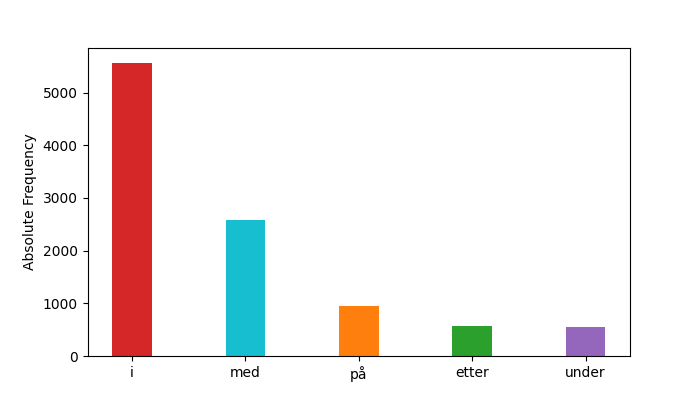
\includegraphics[width=10cm]{pics/barplot_adp_fortsette.png}
    \caption{Five most frequent prepositions introduced by \emph{fortsette}.}
    \label{fig:barplot_pos_fortsette}
\end{figure}

\noindent A more accurate analysis of ADP distribution shown in Figure~\ref{fig:barplot_pos_fortsette} reveals that prepositions \emph{i} is the most prevalent, accounting for approximately 12\% of the semantically canonical sentences with \emph{fortsette} as predicate. Interestingly, the prepositions of our interest, namely \emph{med}, and \emph{på}, are the next common prepositions, with 2,574 and 949 instances respectively, covering only 5\% and 2\% of relative frequency, a significantly smaller sample compared to the first preposition. 

As the aim of this project is to understand how and to what extent complement coercion in Norwegian may arise, also in this subsection we will systematically analyze sentences with the continuation verb combined with prepositional phrases introduced by \emph{på} and \emph{med}. As seen with the previous group of verbs, also in this case the first step is to distinguish and filter sentences introduced by agentive and non-agentive subjects. Table~\ref{tab:fortsette_agentive} illustrates the distribution of sentences categorized by type of subjects, distinguishing between agentive and non-agentive subjects. The data is further divided based on the syntactic composition, namely prepositioanl phrases \emph{på} and \emph{med}, as well as noun phrases. Results  suggests that prepositions do prefer sentences with non-agentive subjects, as being the majority in frequency found. Only a small portion of sentences can be candidate to account for the phenomenon of complement coercion: among approximatively 1,000 senteces introduced by \emph{på}, only 213 sentences presents agentive subjects which covers less than 1\% of the entire verb subsample, while 795 out of 2574 instances are found with the preposition \emph{med}, with 4\% of relative frequency. A contrasting pattern emerges with noun phrases, where 1010 sentence (approximatively one sixth of the subsample) exhibits agentive subjects. 
% \begin{tabular}{llrr}
% \toprule
% {} &     W1 &  VERB &  REL.FREQ \\
% \midrule
% 28 &      i &  5567 &  0.124369 \\
% 44 &    med &  2574 &  0.057504 \\
% 67 &     på &   949 &  0.021201 \\
% 13 &  etter &   563 &  0.012578 \\
% 83 &  under &   553 &  0.012354 \\
% \bottomrule
% \end{tabular}
\subsubsection{Continuation verb with prepositional phrases}
\begin{table}[h]
    \centering
    \begin{tabular}{llrrr}
    \toprule
    Annotation &  på &  med\\
    \midrule
     % ?       &          1 (<0.01) &       0.000022 \\
    entity   &         18($<$0.01) &  244   \\
    event    &         34($<$0.01) &  469   \\
    loc     &        111($<$0.01) &   0  \\
    no      &          1($<$0.01) &  8   \\
    other   &         37($<$0.01)&   35  \\
    skole  &          7($<$0.01) &   na  \\
    temp   &          4($<$0.01) &    10 \\
    \bottomrule
    \end{tabular}
    \caption{Distribution of sentences based on the semantic annotation.}
    \label{tab:fortsette_semantic_adp}
\end{table}
\noindent Table~\ref{tab:fortsette_semantic_adp} shows the sentence distribution of the verb \emph{fortsette} divided by the prepositions \emph{på} and \emph{med} based on the semantic annotation. Results suggests that the instances combined with agentive subjects and the preposition \emph{på} is basically used for introducing locative adjuncts, encompassing the majority of frequency found, with 111 sentences. The next group of sentences are those that introduce event-denoting arguments, with 34 identified sentences. Entity-denoting arguments comprise only 18 sentences. A different situation is found when the continuation verb is followed by the preposition \emph{med}. Event-denoting arguments are the most common occurrence, with 468 instances annotated, while entity-denoting arguments are found only 239 times in the corpus. A comparison between prepositions we can notice that the verb fortsette appears to prefer in both cases event-denoting arguments. Despite its high ranking, entities seems to remains to be infrequent in all cases. 
Among sentences including entity-denoting arguments, the verb \emph{fortsette} presents 11 possible cases of complement coercion. The entity type that we found in the corpus include only an extremely limited amount of artifacts, basically related to medicines, books and money. Sentence~\ref{example_fortsette_paa1} shows for example that the the patient, who has already started a course of drug treatment, continues with the therapy until a specific time specified in the sentence:
        \ea \label{example_fortsette_paa1} %NCC

        \gll Pasienter (...) fortsetter på legemiddelet frem til uke 24 for ny vurdering av effekt.\\
             Patients (...) continue on medicine forth to week 24 for new evaluation of effect.\\
        \glt ‘Patients (...) continue the medicine until week 24 for reassessment of efficacy’
        \z
    
In addition, other types of entity include more abstract terms that mainly concern the continuation of topic discussion, movie production and the prosecution of courses attendance:
        \ea \label{example_fortsette_paa2} %NCC

        \gll Mange studenter fortsetter på samme tema på masteroppgaven (...).\\
             Many students continues on same topic on master's-thesis.\\
        \glt ‘Many students continue on the same topic in their master's thesis’
        \z
Given the previous context, Sentence~\ref{example_fortsette_paa2}, in this case, mentions the fact that many students being involved in group research projects decide to proceed the discussion of the research topic on their master thesis.   
Considering prepositional phrases composed with the preposition \emph{med}, we observe a greater amount of instances suggesting coercion compared to the previous set, with 94 annotated sentences. The entities span here a significantly broader spectrum, including also in this case concrete and abstract terms. Interesting here is the low presence of artifacts and objects of everyday use, mostly related for example to medicine, books, and text:
        \ea \label{example_fortsette_med1} %NCC

        \gll Nesbø fortsetter med «Kakerlakkene» , en riktig ambassadørmix av det bedervede, uhyggelig slaget.\\
             Nesbø continues with «Kakerlakkene», a real ambassador-mix of rotten, spooky kind-the.\\
        \glt ‘Nesbø continues with "Kakerlakkene", a real ambassador mix of the stale, creepy kind.’
        \z
Also with the verb of continuation, the preposition \emph{med} is often combined with food and beverages:
        \ea \label{example_fortsette_med2} %NCC

        \gll Brunchgjestene på Casbah Cafe fortsetter med salaten.\\
             Brunch-guests at Casbah Cafe continue with salad-the.\\
        \glt ‘Brunch guests at Casbah Cafe continue with the salad.’
        \z
Results, on the other hand, suggest a stronger prevalence of more abstract entities of different kind, from continuing to sing songs, play music, asking and answering questions to story telling and anectodes revealings: 
        \ea \label{example_fortsette_med2} %NCC

        \gll Jostein fortsetter med et nytt eksempel på planting.\\
             Jostein continues with a new examples on planting.\\
        \glt ‘Jostein continues with another example of planting.’
        \z
        
%Also here difficulty to distinguish whether coercion, company, modo,mezzo. 
% Also in this case med is used in combination with food. Maybe because food is considered is linked with the act of subevents. 
% We can confirm that med can be used for two reasons:
% 1. use to define a temporal 
% treating a topic
% work on the farm?
% write book
% attend chemitry course
% take medicine
% study BA
% receive money
% Do a remake
%%% PROBLEMS FORTSETTE PAA:
% fortsette på kurs: how to treat it?
% fortsette på prosjekt: always treated as eventive, how to treat it?
% rehabiliteringspenger: how did I treat in the other verbs? Here I would say it could be coercion.
\subsubsection{Continuation verb with direct objects}
\begin{table}[h]
    \centering
    \begin{tabular}{llrrr}
    \toprule
    Annotation &  Noun\\
    \midrule
    entity & 12 & 0.001873 & 0.000268 \\
    event & 1602 & 0.250039 & 0.035789 \\
    other & 32 & 0.004995 & 0.000715 \\
    temp & 119 & 0.018573 & 0.002659 \\
    \bottomrule
    \end{tabular}
    \caption{Distribution of sentences with the verb \emph{fortsette} followed by noun phrases, based on the semantic annotation.}
    \label{tab:fortsette_semantic_noun}
\end{table}
\noindent As previously mentioned, the verb \emph{fortsette} combined with direct object presents a small distribution of sentences combined with agentive subjects. Table~\ref{tab:fortsette_semantic_noun} reveals that the direct objects mostly introduce event-denoting arguments, with 1,602 instances found in the corpus. Apparently, entities are definitively infrequent elements, with only 12 sentences found. Among them, 5 instances could be considered potential candidates for complement coercion. It is interesting to notice that all identified objects do not correspond to proper artifacts, but more abstract terms, revealing interpretations such as course proposals, story telling, and writing books.

\subsection{Verbs of conclusion}
\vspace{1cm}

    \begin{minipage}{.3\textwidth}
      \centering
    \begin{tabular}{llrr}
    \toprule
    \midrule
    Avslutte &  Freq.(rel.freq) \\
    \midrule
    NOUN &  6759(0.305050) \\
    ADP &  5184(0.233967) \\
    OTHER &  3613(0.163064) \\
    PRON &  3284(0.148215) \\
    DET &  1312(0.059214) \\
    SCONJ &  1048(0.047299) \\
    EMPTY &   956(0.043147) \\
    PART &     1(0.000045) \\
    \bottomrule
    \end{tabular}
    \captionof{table}{Frequency distribution of POS introduced by \emph{fortsette}.}
\label{tab:avslutte_POS}
    \end{minipage}%
\hfill
\begin{minipage}{.5\textwidth}
  \centering
\begin{tabular}{llrr}
    \toprule
    \midrule
Ende &  Freq &  REL.FREQ \\
\midrule
ADP &  4863 &  0.640711 \\
OTHER &  1000 &  0.131752 \\
SCONJ &   795 &  0.104743 \\
NOUN &   280 &  0.036891 \\
PRON &   254 &  0.033465 \\
EMPTY &   238 &  0.031357 \\
DET &   144 &  0.018972 \\
PART &    15 &  0.001976 \\
INTJ &     1 &  0.000132 \\
\bottomrule
\end{tabular}
  \captionof{table}{Distribution of sentences based on agentive and non-agentive subjects.}
 \label{tab:ende_POS}
\end{minipage}

\vspace{1cm}

\noindent The last set of verbs that we will analyze consists of cessation verbs \emph{avslutte} and \emph{ende}. A quantitative analysis concerning the POS distribution of the verb \emph{avslutte} reveals that noun is the most frequent part-of-speech, with 6,759 sentences found in the corpus and covering 30\% of the verb subset. Prepositions follow the nouns with more than 5,000 instances, covering 23\% of the subset. Interesting is the almost absence of particles introducing infinitval clauses (PART) that, in comparison with the previous analyzed verbs, we find only one case. The latter verb of cessation, \emph{ende}, shows a slightly different POS distribution. The most frequent word type found in the corpus are prepositions, with almost 5,000 instances, constituting the absolute majority with 64\% of relative frequency. Nouns, on the other hand, seem not to be preferred by the verb, with only 280 instances found (only 3\% of relative frequency). Similar to the previous verb, infinite clauses appear not to be frequently employed with this verb. Only 15 instances are found in the corpus. 
\begin{table}[h]
    \centering
    \begin{tabular}{lrrrr}
        \toprule
        & \multicolumn{2}{c}{\textbf{Avslutte}} & \multicolumn{2}{c}{\textbf{Ende}} \\
        \cmidrule(lr){2-3} \cmidrule(lr){4-5}
        \textbf{} & \textbf{agentive} & \textbf{no agentive} & \textbf{agentive} & \textbf{no agentive} \\
        \midrule
        På &   128(0.03/0.006) & 47(0.01/0.002) & 109(0.02/0.014) & 447(0.17/0.11)\\
        Med      &  601(0.116/0.03) & 1366(0.07/0.02)  & 53(0.012/0.01) &  835(0.17/0.11)\\
        Noun      &  1562(0.24/0.03) & 305(0.05/0.01) & 35(0.01/0.005) &  51(0.01/0.01) \\
        \bottomrule
    \end{tabular}
    \caption{Table Caption Here}
    \label{tab:cessation_verbs_agentive}
\end{table}
\begin{figure}[htp]
    \centering
    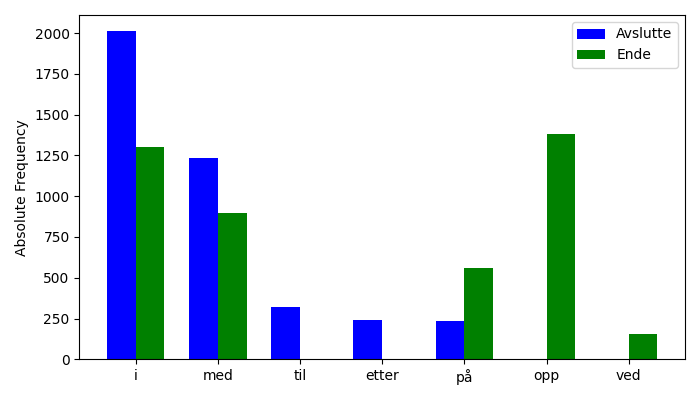
\includegraphics[width=10cm]{pics/barplot_adp_avslutte_ende.png}
    \caption{Five most frequent prepositions introduced by \emph{fortsette}.}
    \label{fig:barplot_pos_fortsette}
\end{figure}
Table~\ref{tab:cessation_verbs_agentive} illustrates the distribution of sentences categorized by type of subjects distinguishing between agentive and non-agentive and further divided by prepositional phrases \emph{på} and \emph{med} and noun phrases. Concerning the verb \emph{avslutte} we observe a prevalence of agentive subjects when encountering direct objects, with 1562 instances, and prepositional phrases introduced by \emph{på}, with 128 sentences. An opposite direction is found with prepositional phrases with \emph{med}, where non-agentive subjects prevails among the other three constituent types. Concerning the verb \emph{ende}, on the other hand, we can notice a different trend in distribution. In every case, this verb would prefer the introduction of non-subjective type. Only few instance with agentive subjects were indentified, with 178 instances combined with \emph{på}, 62 with \emph{med} and 35 with direct objects.  

\subsubsection{Cessation verbs with prepositional phrases}
\begin{table}[h!]
    \centering
    \begin{tabular}{lllll}
        \toprule
        & \multicolumn{2}{c}{\textbf{Avslutte}} & \multicolumn{2}{c}{\textbf{Ende}} \\
        \cmidrule(lr){2-3} \cmidrule(lr){4-5}
        \textbf{Class} & \textbf{på} & \textbf{med} & \textbf{på} & \textbf{med} \\
        \midrule
        \midrule
    entity &         6(0.003/0.0003) & 156(0.03/0.003)&2(0.02/0.01  &   9(0.004/0.003)\\
    event &         19(0.004/0.0004) & 367(0.1/0.01)& 13(0.002/0.001) & 28(0.01/0.004)\\
    loc &         70(0.012/0.001) & 5(0.001/0.0001)&  83(0.02/0.01) & 0(0/0)\\
    other &         25(0.005/0.001) & 10(0.002/0.0002)&  5(0.001/0.001) & 2(0.0004/0.0003)   \\
    temp &          6(0.001/0.0001) & 2(0.0004/0.00004)& 1(0.0002/0.0001)  & 0 (0/0)  \\
        \bottomrule
    \end{tabular}
    \caption{Table Caption Here}
    \label{tab:mytable}
\end{table}
\noindent This corpus analysis also permitted to gain insight into the distribution of sentences combined with cessation verbs and prepositional phrases of our interest. Table \ref{tab:cessation_verbs_agentive} illustrates the sentence frequency divided by semantic annotated classes. The scarsity of sentences featuring agentive subjects, seen before, has led to sparse representation for both verbs, reflecting low amount of outcomes to analyze. Considering, for instance, the distribution of sentences with prepositional phrases introduced by \emph{på}, we can see that the verb \emph{avslutte} would mainly tend to express locative adjucts after the predicate, with 64 instances found, followed by eventive arguments, with 19 sentences. Entity-denoting arguments represents a limited sample with only 14 cases identified in the corpus. Similarly, the verb \emph{ende} demonstrate a preference for combining the preposition with locative adjucts, finding 83 instances. Only 8 instances with eventive arguments were found instead. Compared to the previous verb, we found a higher amount of entity-denoting arguments, with 76 annotated sentences.

From an attentive analysis of sentences found in the corpus we have noticed that the combination of preposition \emph{på} and verbs of cessations does not necessarily lead to cases of complement coercion. Concerning the verb \emph{avslutte}, only one case\footnote{In the corpus we found other four sentences that were very similar. Despite the partial differences in wording between all sentences, they were not considered as duplicates.} could be considered a plausible candidate:
    \ea \label{example_avslutte_paa1} %NCC
    \gll Personer avsluttet på rehabiliteringspenger 1. halvår 1993 (...).\\
         People finished on rehabilitation-money 1st half-year 1993 (...).\\
    \glt ‘People finished (receiving) rehabilitation benefits in the first half of 1993 (...).’
    \z
\noindent From Sentence~\ref{example_avslutte_paa1} it is clear that the subjects is going to terminate receiving a monetary benefit for substenance. 
The verb \emph{ende}, instead appears not have real candidates for complement coercion. All identified entities in sentences were not suitable to occur the phenomenon. An example can be seen in Sentence~\ref{example_ende_paa1}:
    \ea \label{example_ende_paa1} %NCC
    \gll De jentene som ikke tar realfag, ender ofte på medisin eller juss.\\
    The girls-the that not take science-subject, end on medicine or law.\\
    \glt ‘The girls who don't take science subjects often end up in medicine or law.’
    \z
    
Concerning the distribution of semantic annotated sentences combined with the preposition \emph{med}, event-denoting arguments seem to prevail in the sample, with a high frequency of 367 sentence with \emph{avslutte} and, to minor extend, with \emph{ende} with only 27 cases. Entity-denoting arguments follows the previous semantic class, where \emph{avslutte} encompasses 156 cases, while 19 instances were found in \emph{ende}.  
A deeper semantic analysis of sentences with the verb \emph{avslutte}, 105 sentences can be considered plausible candidates of complement coercion. Similar to other cases with this preposition, the sentences include more abstract entities mainly related to eating food, singing songs, play instruments and asking questions:

    \ea \label{example_avslutte_med1} %NCC
    \gll Koret avslutter med "Gud Signe Norigs Land".\\
    Choir-the finishes with "Gud Signe Norigs Land".\\
    \glt ‘The choir ends with "Gud Signe Norigs Land".’
    \z 

Concerning the verb \emph{ende}, on the other hand, seems to not occur complement coercion. A small subset of sentences that combine with entity-denoting arguments do not convey the meaning of completing doing something with the object. Instead, it suggests that the subjects "end up" with the object at hand (example in Sentence~\ref{example_ende_paa1}, therefore excluding any coercion phenomenon:
    \ea \label{example_ende_paa1} %NCC
    \gll En fjerdedel av elevene som i utgangspunktet startet på yrkesfag, ender med studiekompetanse.\\
    A quarter of pupils-the that in starting-point started on profession-subject ends with study-competence.\\
    \glt ‘A quarter of pupils who initially started in vocational education end up with study qualifications.’
    \z

%NOUN
Table~\ref{tab:cessation_semantic_noun} describes the distribution of semantic annotated sentences combined with direct objects. Results reveal an important difference between the two verbs: due to the limited sample size  for the verb \emph{ende}, there is a scarcity of annotated sentence available for the analysis. The majority of sentences, 18 instances, were classified as eventive, covering approx. 10\% of the subset of the entire subset. Only six sentences were annotated as entity. The verb \emph{avslutte}, on the other hand, offers a larger amount of sentences: 21\% of relative frequency of the subset provide the noun phrases as eventive, with 1,323 instances. Entity-denoting arguments, however, appear not to be highly frequent, with only 150 instance (2\% of relative frequency). 


%Some sentences are discarded, mention it somewhere. 

Only two possible candidates for coercion were found with the verb \emph{ende}
%ende N : presence of ende N med.
%avslutte N : presence of avslutte N med. 
\subsubsection{Continuation verb with direct objects}
\begin{table}[h!]
    \centering
    \begin{tabular}{lll}
    \toprule
    Class &  Avslutte & Ende\\
    \midrule
    entity  & 150(0.023/0.003)  & 6(0.02/0.001) \\
    event   & 1323(0.21/0.03)   & 18(0.1/0.002)\\
    no      & 10(0.002/0.0002)  & 1(0.003/0.0001)\\
    other   & 57(0.01/0.001)    & 3(0.01/0.0003)\\
    temp    & 15(0.002/0.0003)  & 3(0.01/0.0003)\\
        \bottomrule
    \end{tabular}
    \caption{Caption.}
    \label{tab:cessation_semantic_noun}
\end{table}
Analyzing the verb \emph{avslutte}, only a limited set of sentences can be considered cases of complement coercion, counting a total amount of 7 sentences. The type of entities found varies from real artifacts such as poetries, letters but also more abstract terms (attending courses):
    \ea \label{example_avslutte_noun1} %NCC
    \gll Han avsluttet diktet våren 1818 i Devonshire, nedråtnet i regnvær.\\
    He finished .\\
    He finished poem-the spring-the 1818 in Devonshire, decomposed in rain.
    \glt ‘He finished the poem in the spring of 1818 in Devonshire, decomposing in the rain.’
    \z
The context provided in sentence~\ref{example_avslutte_noun1} mentions the fact that the subject concluded writing the poem. 
Regarding the verb \emph{ende}, it appears that when combined with noun phrases, this verb is not basically used to elicit, as no candidate sentences were found.


%Problem with skole - how to treat them? 
%Avslutte N med./slik
%one case where avslutte has synonym of close.  
%Avslutte NOUN - is not so much used. See Spalek
% \subsubsection{Cross-linguistic comparion with Dutch, German and English}

\newpage



% \bibliographystyle{alpha}
% \bibliography{sample}

% \printbibliography

\end{document}


% appunti su avslutte:
a quanto pare è un verbo che non venga utilizzato  moltissimo
avsutte boken ok
avslutte spillet ok
avslutte pizza no
avslutte albumet

a quanto pare viene utilizzato spesso per inidicare ultimazione di un argomento che abbia telicità e che ci sia incrementalità.
preferenza di utilizzo di altri verbi. 
avslutte altri sinomini: spegnere. 

# begynne med vs paa: a parte la questione di sottoevento, sembra che lo si usi anche quando non si ha intenzione esplicita di un sottoevento.

gutten begynne med  il fatto che si usi med potrebbe essere riferito a preferenza di scrivere vs leggere? su Sprakspalta
si è creato un dibattito tra madrelingua ma a quanto pare non c'è una differenza evidente. Userebbero entrambi senza distinzione. 
Una possibilità potrebbe essere sempre legata al sottoevento o qualcosa di simile: 
- begynne med boken (che in italiano non suonerebbe bene come in norvegese) significa avere a che fare con il libro. Probabile che med possa essere piu accettabile qualora ci sia già stata citata l'intenzionalità del soggetto a fare una determinata azione che poi non viene menzionata senza dare troppa enfasi sull'argomento. La preposizione på, invece, pare dare quell'enfasi che triggera la coercion. 
begynne på boken - potrebbe indicare che il soggetto (per esempio intenzionato alla scrittura) crei il libro. 
Sarebbe carino creare un esperimento con un determinato contesto per poter vedere se ci sia una differenza tra på e med oppure vengono utilizzati in maniera intercambiabili

difficile trovare una cosa simile con il verbo avslutte. 













CONCLUSIONE:
FROM VERSPOOR:
What is strongly suggested by the data introduced in the previous section is that the metonymic construction is only used with the aspectual verbs begin and finish if the intended event is a strong default associated with the noun phrase. vorrei usare questa frase per idicare una tendenza ad utilizzare PP con i verbi di iniziazione. Un possibile utilizzo pare possa esserci anche con NP anche se non è possibile notarlo qua. Può darsi che la marca preposizionale sia utikizzata per dare più enfasi all'evento.  mentre senza non sarebbe possibile. 



%APPENDIX:
% -creation of table of distribution of ADPs (and also single prepositions) and NOUNS across verbs. 
